\subsection{Neural Net Definitions}

Here we look into a neural network based on perceptron cells with an activation function.
A single perception can be regarded as a linear classifier, i.e. it is able to output
which of two linearly separable data sets a given point belongs to. In order to classify
more complex data sets, layers of perceptrons with non-linear activation functions are
required.

\begin{figure}[h] \centering
    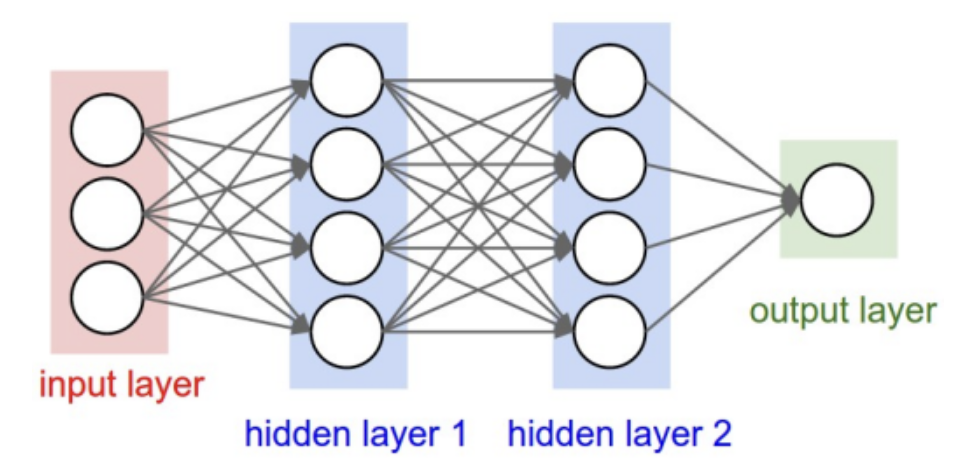
\includegraphics[width=0.75\textwidth]{neural_network} \caption{A fully
    connected multi-layer neural network with three inputs, two
    hidden layers, each with four perceptron nodes and an output layer with a
    single output node. (Source: https://towardsdatascience.com)} \label{fig:neural_network}
\end{figure}

A neural net consists of $L$ layers with $n^l$ nodes in each layer $l=[0,L)$. For the
input layer $(l=0)$ the nodes are simple input nodes, while for the remaining layers
consist of perceptron nodes (see figure~\ref{fig:percptron}). \\

A perceptron with an arbitrary activation function looks like this:
\begin{figure}[h] \centering 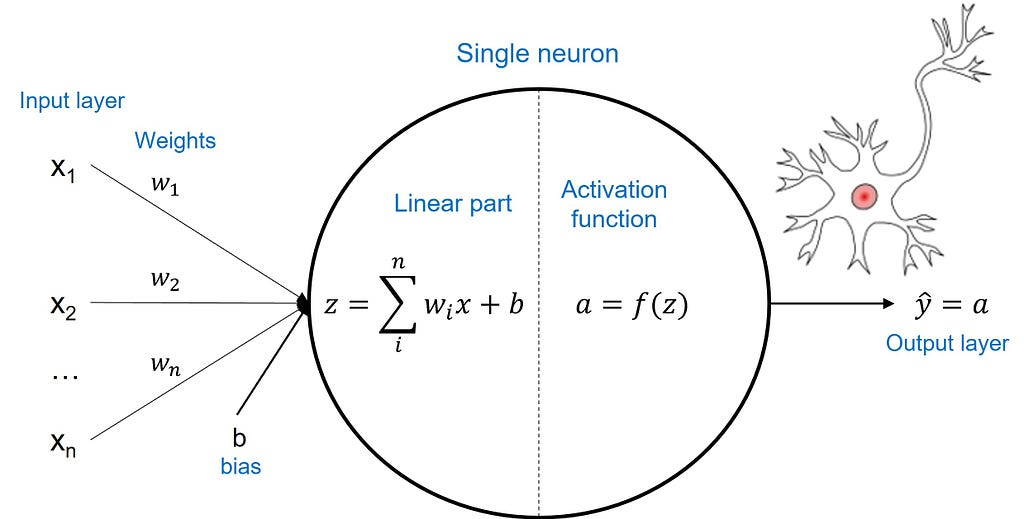
\includegraphics[width=0.75\textwidth]{single_neuron}
    \caption{A node of a neural network with inputs, bias and activiation function.
    (Source: https://towardsai.net)}
    \label{fig:percptron}
\end{figure}

Definitions:
\begin{enumerate}
    \item The training dataset $X$ consisting of input-output pairs $(\vec{x}_i,
    \vec{y}_i)$, where $\vec{x}_i$ is the input and $\vec{y}_i$ is the desired or target
    output of the network on the input $\vec{x}_i$. The set of input-output training pairs
    of size $N$ is denoted $X = \{(\vec{x}_1,\vec{y}_1), \dots, (\vec{x}_N,\vec{y}_N)\}$.

    \item A feedforward neural network has (learning) parameters, i.e.\ weights and
    biases, that are collectivly denoted $\theta$. The nodes in different layers are fully
    connected, while there are no connections between nodes in the same layer. For
    backpropagation the parameters of primary interest are $w^l_{tf}$, the
    weight\footnote{In this notation the index $t$ stands for \emph{to}, whereas $f$
    stands for \emph{from}. Index $t$ always refers to nodes in layer $l$, while index $f$
    always refers to nodes in layer $l-1$.} between the node with index $t$ in layer $l$
    and the node with index $f$ in layer $l-1$, and $b^l_t$, the bias of the node with
    index $t$ in layer $l$. 

    \item A loss function $L(X,\theta)$, which defines a quantitative measure for the
    error between the desired output $\vec{y}_i$ and the calculated actual output
    $\vec{a}^l_i$ of the neural network on the input $\vec{x}_i$ for an input pair
    $(\vec{x}_i, \vec{y}_i) \in X$ and a particular value of the learning parameters
    $\theta$.
\end{enumerate}

Following values are used to define the network:
\begin{itemize}
    \item $x_t$, the input at index $t$ of an input vector $\vec{x}_i$ of the training set
    in the input layer ($x_t = a^{l=0}_t$ after activation of the input layer in the
    implementation, see below for definition of $a^l_t$).

    \item $w^l_{tf}$, the weight between the node with index $t$ (\emph{\underline{t}o})
    in layer $l$ and the node with index $f$ (\emph{\underline{f}rom}) in layer $l-1$.

    \item $b^l_t$, the bias of the node with index $t$ in layer $l$.
    
    \item $z^l_t = \sum_{f}{w^l_{tf} a^{l-1}_f} + b^l_t$ is the total input the node gets
    from the activated nodes of the previous layer and it's bias.
    
    \item Activation functions $f_h$ for the \underline{h}idden layers and the
    \underline{o}utput layer $f_o$.
    
    \item The activation $a^l_t$ at index $t$ in layer $l$. $a^l_t = f_h(z^l_t)$ in hidden
    layers or $a^{L-1}_t = f_o(z^{L-1}_t)$ for the output layer. The activation function
    for the input layer is the identity function in the implementation.

    \item $a^{L-1}_t$ is the output component at the index $t$ in the output layer at the
    given input $\vec{x}_i$. The intended output is defined by $\vec{y}_i$ as second part
    of the training pair $(\vec{x}_i, \vec{y}_i)$, where $y_t$ is component $t$ of
    $\vec{y}_i$.
\end{itemize}

The activation functions are chosen to fit the needs of the application. The nodes in the
\underline{h}idden layers $l=1$ up to $l=L-2$ have an activation function $f_h$ while the
nodes in the \underline{o}utput layer $(l=L-1)$ might have another acitivation function
$f_o$. \\

The loss function is also chosen as best fit the to problem at hand. The goal of training
of the network is to minimize the loss function and thus to minimize the remaining error
for a given set of training data. Gradient descent is used to reduce the error during
training. A typical example of a loss function is the quadratic cost function (mean
squared error with additional factor of $frac{1}{2}$ to make the derivative calculation
easier).
\begin{equation}
    L(X,\theta) = \frac{1}{2N} \sum_{t=0}^{N-1}{\lVert a^{L-1}_t - y_t \rVert^2} = \frac{1}{2N} \sum_{t=0}^{N-1}{(a^{L-1}_t - y_t)^2}
\end{equation}
In order to minimize the loss function, we need to understand how the deviation of the
actual output to the desired output depends on the choice of learning parameters $\theta$,
i.e. the weights $w$ and the bias values $b$. In order to minimize the the loss function,
and thus the deviation between acutal and desired output, they have to be changed in a
direction against the gradient of the function $L$. This requires to calculate all partial
derivatives of the loss function with respect to the weights $\pd{L}{w}$ and with respect
to the biases $\pd{L}{b}$.\\

To understand why this is the case let's consider:


% \emph{Basis transformation:} The basis vectors of the new system expressed as a linear
% combination of the basis vectors of the old system is considered a forward transformation.
% The other direction is considered a backward transformation.\\

% Here $F$ stands for $\underline{F}$orward transformation. Basis vectors are chosen to be
% left multiplied to the transformation matrix, corresponding to summation via the first
% index of the transformation matrix. Indices are chosen upper and lower to enable the
% Einstein summation convention later on. Transformation indices are always from "north
% west" to "south east":
% \begin{equation}
%     \label{eq:forward_trafo}
%     \begin{array}{rcl}
%         [\hdbtv{1} \quad \hdbtv{2}] & = &
%         [\hdbv{1} \quad \hdbv{2}]
%         \begin{bmatrix}
%             F^{1~}_{~1} & F^{1~}_{~2} \\
%             F^{2~}_{~1} & F^{2~}_{~2}
%         \end{bmatrix} \\
%         \noalign{\vskip10pt}
%         \hdbtv{1} & = & F^{1~}_{~1}\hdbv{1} + F^{2~}_{~1}\hdbv{2}
%         \quad \underset{\text{figure}~\ref{fig:old_new_base}}{=} \quad
%         2 \hdbv{1} + 1 \hdbv{2} \\
%         \hdbtv{2} & = & F^{1~}_{~2}\hdbv{1} + F^{2~}_{~2}\hdbv{2}
%         \quad \underset{\text{figure}~\ref{fig:old_new_base}}{=} \quad
%         -\frac{1}{2}\hdbv{1} + \frac{1}{4}\hdbv{2} \\
%         \noalign{\vskip10pt}
%         \Rightarrow \hdbtvc{j} & = &
%         F^{k~}_{~j} \hdbvc{k} \quad\text{(summation convention)}
%     \end{array}
% \end{equation}

% Here $B$ stands for $\underline{B}$ackward transformation:
% \begin{equation}
%     \label{eq:backward_trafo}
%     \begin{array}{rcl}
%         [\hdbv{1} \quad \hdbv{2}] & = &
%         [\hdbtv{1} \quad \hdbtv{2}]
%         \begin{bmatrix}
%             B^{1~}_{~1} & B^{1~}_{~2} \\
%             B^{2~}_{~1} & B^{2~}_{~2}
%         \end{bmatrix} \\
%         \noalign{\vskip10pt}
%         \hdbv{1} & = & B^{1~}_{~1}\hdbtv{1} + B^{2~}_{~1}\hdbtv{2}
%         \quad \underset{\text{figure}~\ref{fig:old_new_base}}{=} \quad
%         \frac{1}{4} \hdbtv{1} + (-1) \hdbtv{2}\\
%         \hdbv{2} & = & B^{1~}_{~2}\hdbtv{1} + B^{2~}_{~2}\hdbtv{2}
%         \quad \underset{\text{figure}~\ref{fig:old_new_base}}{=} \quad
%         \frac{1}{2}\hdbtv{1} + 2 \hdbtv{2} \\
%         \noalign{\vskip10pt}
%         \Rightarrow \hdbvc{i} & = &
%         B^{j~}_{~i}\hdbtvc{j}\quad\text{(summation convention)}
%     \end{array}
% \end{equation}

% Between $B$ and $F$ following relation holds:
% \begin{equation}
%     \label{eq:forward_backward_inverse}
%     \begin{array}{rcl}
%         B^{j~}_{~i} F^{k~}_{~j} & = & F^{k~}_{~j} B^{j~}_{~i}
%         = \delta^k_i =
%         \begin{cases}
%             1, & \text{if}\ i = k \\
%             0, & \text{if}\ i \neq k
%         \end{cases} \\
%         \text{full equation transposed:} & = &
%         B^{i~}_{~j} F^{j~}_{~k} = \delta^i_k \\
%         \noalign{\vskip10pt}
%         \Rightarrow B & = & F^{-1} \quad\text{($B$ is the inverse of $F$)}
%     \end{array}
% \end{equation}


\newpage
